% This is a sample LaTeX input file.  (Version of 9 April 1986)
%
% A '%' character causes TeX to ignore all remaining text on the line,
% and is used for comments like this one.

% Rob Phillips lifted from /usr/local/lib/tex/inputs/sample.tex
% to use as template.

\documentclass[12pt]{article}    % Specifies the document style.

 \usepackage[pdftex]{graphicx}
\input{epsf}

\usepackage{fancyhdr}
\usepackage{extramarks}
\usepackage{amsmath}
\usepackage{amsthm}
\usepackage{amsfonts}
\usepackage{tikz}
\usepackage{tcolorbox}
\tcbuselibrary{breakable}
\usepackage{mathtools}
\usepackage{color,soul}
\usepackage{mdframed}
\usepackage{graphicx}
\usetikzlibrary{automata,positioning}
\usepackage{environ}
\usepackage{hyperref}

                           % The preamble begins here.
\begin{document}           % End of preamble and beginning of text.
\relax


\begin{center}
{\bf\Large Bi/Ge105: Evolution}\\
{\bf\Large Homework 2}\\
{\bf\Large Due Date: Thursday, February 1, 2018}\\
\end{center}
 
``Whatever you can do, or dream you can do, begin it.  Boldness has genius, power
and magic in it.''  - Johann Wolfgang von Goethe\\


\noindent {\bf 1. A feeling for the numbers in evolution continued}\\

\noindent The processes of evolution take place at many different scales in
both space and time.  Like last week, the goal of this first problem is nothing more than to ``play''
with some of the characteristic scales associated with a broad range of processes in
evolution ranging from the very small (e.g. number of mutations per cell in a bacterium
after one round of replication) to the very large (e.g. how far do the Galapagos islands travel
in a million years).  These estimates are intended to be done using simple arithmetic of
the ``one-few-ten'' variety (i.e. few times few is ten) and to give an order-of-magnitude 
picture of the phenomenon of interest.  Take pride in  your results and state and
justify (with citations) the assumptions you make carefully and give a simple, intuitive description of how you came
to your results.   Please don't report
rough estimates with long lists of ``significant'' figures.  \\



(a) Genomes are one of the most interesting features of ``living matter''.   One question of interest is the extent to which the ``space'' of possible genomes and gene products has been explored over the history of life.  In a very interesting article by Whitman {\it et al.} called
``Prokaryotes: the unseen majority'', we learn of the vast numbers of bacteria on Earth, with the current estimate coming in at something like $10^{30}$ bacteria.  The number of
viruses is even greater with the so-called ``virus to bacterium ratio'' having a value of roughly 10, implying something on the order of $10^{31}$ phages on earth, suggesting that these viruses are the largest genomic reservoir on our planet.  If we assume that over
more than 3 billion years, these viruses have been steadily replicating in their cycle of infection and lysis, how many total viral genomes have there been in the history of life?  (Obviously, this is a very rough estimate).  Now, compare this number to the number of {\it possible} viral genomes, assuming that each viral genome is 50,000 bp in length.  What
does this estimate tell you about the extent to which sequence space has been explored?
Note: do the approximations, errors and uncertainties in our estimates have any bearing on
our conclusions here?\\

%(b) One of the themes we are going to come back to repeatedly
%is the enormity of sequence space in biology.  As a warm up
%exercise in that regard, in this problem we are going to think
%about the space of possible proteins.  
% In a 2001 Bioengineering seminar, Professor Frances Arnold made a startling
%remark regarding the astronomical number of  possible protein sequences.  In this problem we would like you to generate some intuition for the astronomical number of ways of
%choosing amino acid sequences.  To drive home this point, Prof.
%Arnold noted that if we consider
%a protein with 300 amino acids, there will be a huge number of different possible
%peptide sequences.   Compute how many different sequences there are for a 300 amino acid protein?\\
%
% \noindent   While interesting, this wasn't the shocking part.  Prof. Arnold's provocative remark  was that if we took
%only one molecule of each of these different possible proteins, it would take a volume
%equal to five of our universes to contain all of these different {\it distinct} molecules.
%Estimate the physical size of a protein with 300 amino acids.  Justify your result, but remember
%it is an estimate.  Next, find an estimate of the size of the universe and figure out
%whether Prof. Arnold made a reasonable statement.  Was her estimate of the volume of
%all of these possible proteins too large or too small?\\

(b) Mutations are thought to be one of the main genomic ingredients of evolution.
Given that the bacterial mutation rate is of order $10^{-9}$ per bp per replication, how many
single base pair mutations do you expect to see in a 5 mL tube of bacteria that is saturated
after an overnight culture?  First,
given a roughly 20 minute doubling time, figure out how many cells you expect
in such a culture after 12 hours given that you started with
only a single cell.   Then,  use the replication error rate quoted above,
and make an estimate of how many times each possible point mutation in the
bacterial genome will be found in that culture.  \\

(c) We talked about the diversity of the living world in class,
but with a distinctly macroscopic perspective that focused on
organisms such as insects and animals.  What
about our knowledge of the diversity of the
microbial world?  Every time an electron microscope is used to take an image
it corresponds to roughly a 1$\mu$m $\times$ 1$\mu$m area.
The electron microscope is used to explore the structure
of the nanometer scale world of cells, for example.  Biology
is a subject characterized by great naturalist voyages in
which figures such as Humboldt, Darwin, Wallace, Huxley
and Hooker traveled around the world to try and collect data on
biological diversity.  The point of this problem is to get  a sense of
the {\it microscopic} diversity explored.  Make an estimate of
the total area looked at in biological samples using electron microscopes
in the history of science.  How does this correspond to the area of
the Earth?  What do you conclude about the extent to which
we have ``explored'' the microbial diversity on the planet?\\


\noindent {\bf 3. How Did Frogs Get to S\~{a}o Tom\'{e}?}\\


In class we discussed the fascinating example of the frogs of S\~ao Tom\'e as a
compelling story in biogeography.  In this problem, we will explore in more
detail the way that DNA sequence was used as a window into the dispersal of
these frogs onto these oceanic islands.\\

S\~ao Tom\'e is an island located 255 km off the west coast of Africa. Volcanic
activity formed this island roughly 13 million years ago, and continued to shape
the landmass until as  recently as the last hundred thousand years.
Nevertheless, due to their considerable distance from the African coast and how
recently they emerged from beneath the surface of the water, the islands in the
Gulf of Guinea are  a clear example of biodiversity due to dispersal. While
birds may have flown to the island and seeds may have dispersed via birds or
storms carrying them, the question of how amphibians traversed such far
distances is harder to resolve for reasons having to do with their low saline
tolerance. To understand just how challenging this journey is, in this problem
we will compare the \emph{Ptychadena newtoni} species to other \emph{Ptychadena}
species to determine  the S\~ao Tom\'e inhabitant's origin.\\
\\
\newline
\textbf{Enter the Sequence Revolution?}\\

As illustrated in class, DNA sequencing is a powerful tool to determine the
phylogenetic relationship between similarly related species, but in order to
generate precise results,  the DNA region(s) to sequence must be carefully
chosen. Highly conserved regions of the genome such as the molecules associated
with the central dogma. In the problem posed here, we will use the
popularly-chosen 16S ribosomal RNA region on mitochondrial DNA. \\

(a) Write several sentences explaining what mitochondrial DNA is and
what 16S ribosomal RNA is doing in the mitochondrial genome.\\

The seemingly endless array of sequences openly available through various
databases make it possible to access sequences of all kinds. With such a vast
number of sequences, there is a need to organize them so that they can be easily
manipulated,  leading to a variety of standard formats. With this homework, you
have been given sequence files relevant to the different \emph{Ptychadena}
species in a well known format known as FASTA.  For this assignment you will
have  two .txt files provided with the homework.  You will see that each
sequence in a given  file is composed of a line (beginning with a ``$>$''
symbol) containing information about the sequence, i.e. the species name, the ID
number for obtaining the sequence from a particular database  and, as we have
provided here, the location of the species.  The subsequent lines before the
next ``$>$'' contain the sequence. We have already  aligned the sequences by
placing gaps (`\texttt{-}')  in each of them, making it easy to compare each
sequence directly. \\

While one of the files contains 16S mitochondrial DNA sequences from 26
different species scattered throughout mainland Africa, the other file contains
the sequences of three amphibians of the same species on S\~ao Tom\'e. Because
there may be some variation in the sequence of DNA across individuals within the
same population,  it is often useful to collect samples from multiple
individuals of the same species  to provide stronger evidence for the
relationships of the species with others. In this assignment, you should find
that, not surprisingly, the three \emph{Ptychadena newtoni} on S\~ao Tom\'e
agree well with each other in their relationships to the \emph{Ptychadena}
species across mainland Africa.\\
\\
\\
\\
{\bf{Comparing Frog Sequences.}}\\

(b)  Using what you learned in the computational tutorial for
this week, write a function that directly compares two sequences and assigns a
score. There are a variety of scoring systems for comparing sequences, so for
this problem, create a system where the score  is the number of matches between
two sequences divided by the number of positions compared. If at any position,
either one of  the sequences has a gap `-', ignore that position in the
scoring.   Once you have written your function, compare each S\~{a}o Tom\'{e}
sample's sequence 	to that of each mainland African species and identify the
best three matches, verifying that the three S\~{a}o Tom\'{e} samples agree in
their top three matches. Locate the regions of Africa of these three frog
species.\\

You should only need BioPython's SeqIO and maybe NumPy's zeros function for this
problem. {\it Hint: refer to Tutorial for additional guidance.}\\

\begin{figure}[h!]
	\centering{
		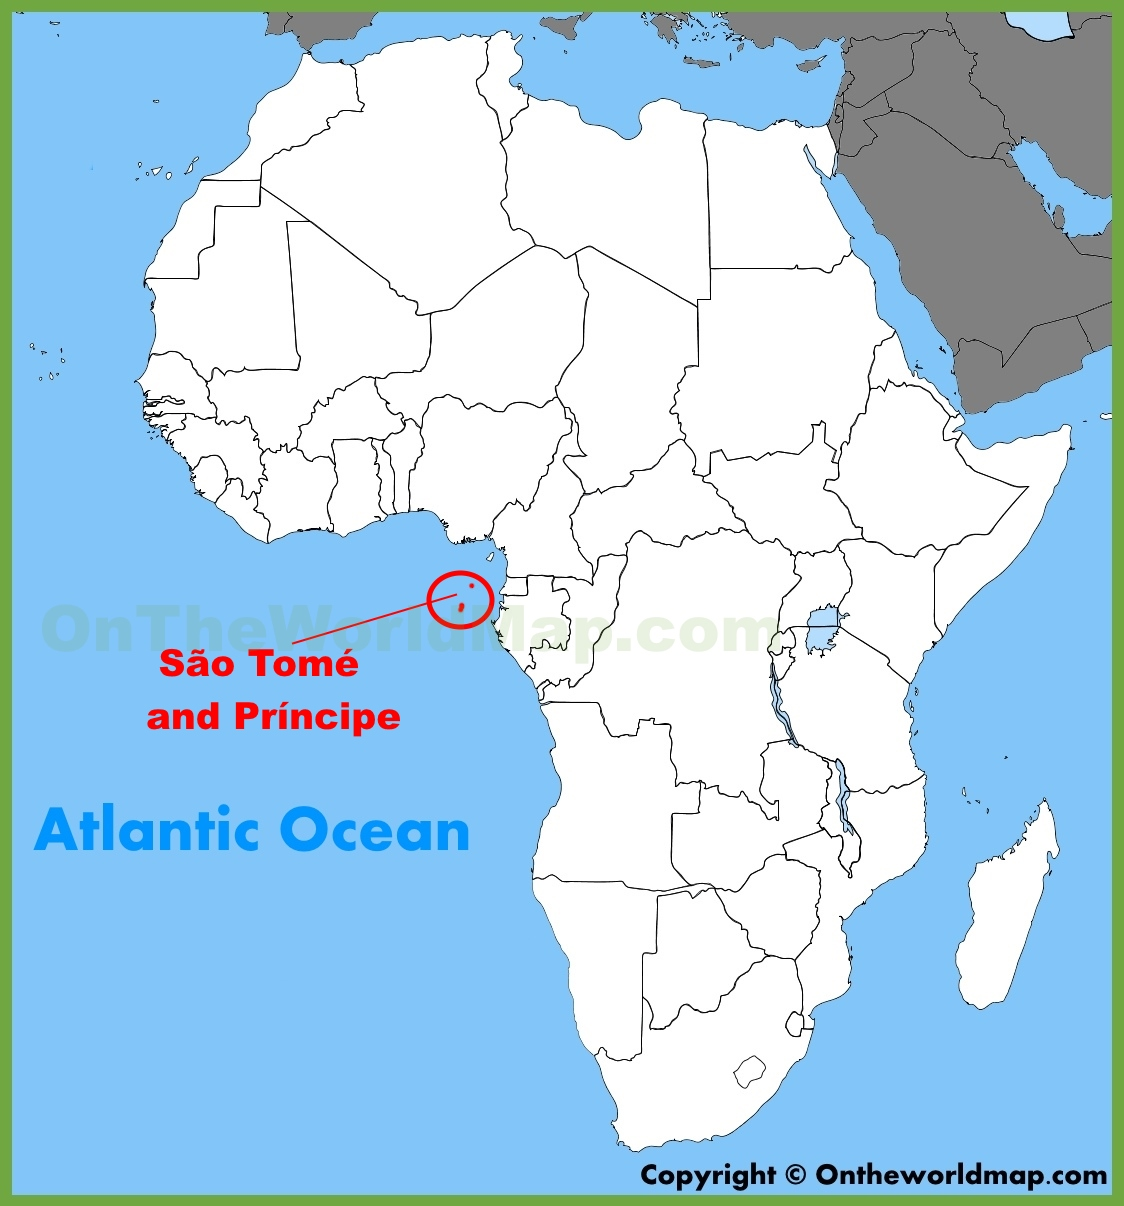
\includegraphics[scale=0.4,trim={0cm 0cm 0cm 0cm}]{./sao-tome-and-principe.jpeg}}
	\caption{Map of Africa with S\~ao Tom\'e and Pr\'incipe in the red circle.}
	\label{fig:africa}
\end{figure}

{\bf{Can ``Rarely'' Over Short Time Scales Lead to ``Frequently'' Over Long Time
Scales?}}\\

In class, we argued that one of the key points of the class is to talk about the
great principles of biology. Obviously, a contender for most important principle
of all is that of the theory of evolution. One of the pieces in the evolution
puzzle is the challenge of trying to make sense of what Alfred Russel Wallace
discovered about the distribution of different organisms in both space
(biogeography) and time (fossil record). In this part of the problem, we will
apply our street-fighting mathematics skills to acquaint ourselves with some of
the arguments that have been made for the dispersal hypothesis.\\

Dispersal biogeography has been pejoratively referred to as ``a science of the
improbable, the rare, the mysterious, and the miraculous.'' Our goal in this
problem is to see if we agree with that assessment or if George Gaylord Simpson
had it right when he argued that people have little intuition for accumulated
weight of rare events that play out over very long time scales. Concretely, we
will try to estimate how often amphibians would successfully colonize the
islands in the Gulf of Guinea.\\

Here, we advise you make your estimates for the probability of a successful
colonization event by using what Sanjoy Mahajan in his great book {\it Street
Fighting Mathematics} refers to as ``divide and conquer''.  What this means is
that you take the overarching problem and then divide it into ever smaller sub
problems each of which you can figure out.  For example here, we need to figure
out how many frogs end up in the Gulf of Guinea from the Congo River.  But to
know that, we have to in turn figure out how much of the land adjacent to rivers
such as the Congo River gets flooded during the biggest flooding events. Then,
we might want to estimate the frequency with which trees end up in rivers that
might serve as rafts, etc. Useful resources could include the map in
Figure~\ref{fig:africa},  Google Maps and Earth Nullschool.\\

(c) Based on your results from the DNA sequences, from which
part of Africa would you conclude the \emph{Ptychadena newtoni} originated? If
we accept that proposition, let's now try to understand the challenges of such a
colonization event. Apply the street-fighting mathematics that you used in the
previous problem to see how many groups of amphibians from these parts of
mainland Africa will make it to S\~ao Tom\'e over the 13 million years of the
island's existence.\\


\begin{figure}[h!]
	\centering{
		\includegraphics[scale=0.7,trim={1.4cm 4cm 0cm 4cm}]{./map_africa_rivers.pdf}}
	\caption{Map of Africa and water sources.}
	\label{fig:africa_water}
\end{figure}



\noindent {\bf 3. The place of evolution in biology}\\

In the title to a famous article, Theodosius Dobzhansky noted that ``Nothing in Biology Makes Sense Except in the Light of Evolution''.  In class we discussed a variety of examples of how Darwinian thinking and evolutionary principles influence other areas of the life sciences (e.g. agriculture, medicine, biotechnology).  Research and describe a modern day example of how evolutionary theory has been incorporated into other biological disciplines.  Explain the topic/problem and your thoughts on how evolutionary principles/thinking were applied.  Your brief essay should be 1-2 paragraphs.  Please submit by email in pdf
form to Profs. Orphan, Phillips and the TAs.\\



    \end{document}             % End of document.
